\documentclass[
    a4paper,
    keeplastbox,            % Prevents problems with last line in references
    hyphens,                % Allow hyphenation in \url
%     nospread,               % Suppress whitespace fill for column balancing
    boxit,                  % Show margins (debug only)
]{jacow}

\usepackage{graphicx}       % Extended support for \includegraphics
\usepackage{tikz}           % Powerful drawing package, part of pgf

\usepackage{mathptmx}       % Mathematical PostScript fonts
\usepackage{amsmath}        % General mathematical symbols
\usepackage{textcomp}       % Text companion fonts
% \usepackage[euler]{textgreek}      % text greek letters

\usepackage{enumitem}       % For more control over list parameters.
% Consider using Itemize, Enumerate, Description

% PGF and TikZ definitions for this paper

% TikZ library imports
\usetikzlibrary{positioning}        % Anchor placement support
\usetikzlibrary{calc}               % Coordinate calculations
\usetikzlibrary{shapes.geometric}   % cylinder
\usetikzlibrary{shapes.arrows}      % arrow shapes
\usetikzlibrary{shapes.multipart}
\usetikzlibrary{fit}                % Fitting outline to shape
\usetikzlibrary{arrows}
\usetikzlibrary{arrows.meta}
\usetikzlibrary{shadows}


% Define our colours
\colorlet{normal colour}{green!60!blue!20}  % Normal coloured filled areas
\colorlet{accent colour}{orange!25}         % Accented filled areas
\colorlet{background colour}{black!10}      % Background groups
\colorlet{data colour}{black!50}            % Data flow
\colorlet{trigger colour}{black!80}         % Trigger lines
\colorlet{control colour}{blue!50}          % Other lines etc


% Common TikZ definitions
\tikzset{
    % This seems a reasonably comfortable arrow shape
    >=stealth,
%
    % Define a set of styles
    % First some fills
    background fill/.style={fill=background colour},
    highlight fill/.style={fill=normal colour},
    accent fill/.style={fill=accent colour},
    % Next some lines
    bus/.style={draw, color=data colour, text=black, line width=0.6mm, ->},
    control/.style={color=control colour, text=black, very thick, ->},
%
    % Used for creating an exact fit to an existing list of objects
    tight fit/.style={fit=#1, inner sep=0, line width=0},
    % We almost always want centre aligned node text
    every node/.style={align=center},
%
    box/.style={
        draw, rectangle, very thick, highlight fill,
        minimum width=1.5cm, minimum height=1.1cm},
    small box/.style={
        draw, rectangle, thick, highlight fill},
    component/.style={
        draw, rectangle, thick, accent fill,
        minimum width=11mm, minimum height=8mm},
    buffer/.style={
        regular polygon, regular polygon sides=3, anchor=center,
        accent fill, thick, draw},
    generate/.style={
        background fill, thin, draw=gray,
        copy shadow={
            shadow xshift=1ex, shadow yshift=-1ex}},
%
    trigger line/.style={thin, trigger colour},
    trigger/.style={
        trigger line, >={Triangle[open, scale=1.2]}, shorten >=-5pt, ->},
    trigger dot/.style={fill, circle, inner sep=1pt, line width=-1pt},
    mul/.style={
        draw=black, circle, thick, highlight fill, inner sep=0.5ex},
%
    inline text/.style={
        baseline=(current bounding box.base),
        every node/.append style={anchor=base, font=\scriptsize},},
%
    pics/buffer/.style args={#1/#2}{
        code={
            \draw [thick, -, black] (0.5mm,-2mm) -- (0.5mm,2mm);
            \draw [thick, -, black] (-0.5mm,-2mm) -- (-0.5mm,2mm);
            \node at (0,2mm) [
                rotated anchor=-90, font=\scriptsize, inner sep=0.2em] {#1}
            node at (0,-2mm) [
                rotated anchor=90, font=\scriptsize, inner sep=0.2em] {#2};}},
}


% New tikz key definitions to control behaviour of \multipath.
\tikzset{
    % Default colour for multipath background
    multipath background/.initial=white,
    multipath margin/.initial=0.3mm,
}

% Draws multiple paths with an outline on each path.  Call with path options as
% first optional argument and with a list of paths as the second argument.
\newcommand{\multipath}[2][]{
    \begin{scope}[#1]
        % Pick up multipath margin and background definitions
        \newcommand{\margin}{\pgfkeysvalueof{/tikz/multipath margin}}
        \newcommand{\background}{\pgfkeysvalueof{/tikz/multipath background}}

        % Draw a white background a bit larger than the programmed line
        % thickness.  We turn off any arrows and shorten the line a trifle to
        % avoid any erosion of the endpoints.
        \begin{scope}[
            line width=\pgflinewidth+\margin, color=\background,
            shorten >=\margin, shorten <=\margin, -]
        #2
        \end{scope}

        % Now draw the target path with its original options.
        #2
    \end{scope}
}

% Special coordinates along edge of box
\newcommand{\northcoord}[3]{
    \coordinate (#1 #2) at ($(#1.north west)!#3!(#1.north east)$)}
\newcommand{\eastcoord}[3]{
    \coordinate (#1 #2) at ($(#1.south east)!#3!(#1.north east)$)}
\newcommand{\southcoord}[3]{
    \coordinate (#1 #2) at ($(#1.south west)!#3!(#1.south east)$)}
\newcommand{\westcoord}[3]{
    \coordinate (#1 #2) at ($(#1.south west)!#3!(#1.north west)$)}


% Trick for reusing last coordinate
\makeatletter
\newcommand\lastcoord{\the\tikz@lastxsaved,\the\tikz@lastysaved}
\makeatother


% It's convenient to have a background layer
\pgfdeclarelayer{background}
\pgfsetlayers{background,main}



% ------------------------------------------------------------------------------
% This frightening looking code is used to compute an anchor that rotates with
% the entire picture.  This is useful when anchoring a node in a pic that itself
% will be rotated.
%   Some really tricky code taken from stack overflow question here:
%
%   https://tex.stackexchange.com/questions/128565/
%       how-to-allow-labels-anchors-in-tikz-to-be-affected-by-
%       rotations-without-rotatin

% \pgfmath@smuggleone
%
% Smuggle a macro outside a group.
%
% Changed by TT: Speedup by insisting, that smuggleone is directly
% followed by \endgroup
%
\makeatletter
\def\pgfmath@smuggleone#1\endgroup{%
  \expandafter\endgroup\expandafter\def\expandafter#1\expandafter{#1}}

\let\pgfmathsmuggle=\pgfmath@smuggleone
\makeatother

\tikzset{
    rotated anchor/.code=%
        \begingroup
            \pgfcoordinate{qrr@origin}{\pgfpointorigin}%
            \pgfcoordinate{qrr@direct}{\pgfpointpolarxy{#1}{1}}%
            \pgftransformreset
            \pgfmathanglebetweenpoints{%
                \pgfpointanchor{qrr@origin}{center}}{%
                    \pgfpointanchor{qrr@direct}{center}}%
            \pgfmathsmuggle\pgfmathresult
        \endgroup
    \tikzset{anchor/.expanded=\pgfmathresult}%
}

% ------------------------------------------------------------------------------

% vim: set filetype=tex:
       % Common PGF & TikZ configuration

\newcommand\smallbox[2][small box]{\tikz [inline text] \node [#1] {#2};}


\hyphenpenalty 4000         % Tone down hyphenation


\begin{document}
\title{A New Transverse and Longitudinal Bunch by Bunch Feedback Processor}
\author{
    M.G.~Abbott, G.~Rehm, Diamond Light Source, UK; I.S.~Uzun, STFC, UK}
\maketitle

\begin{abstract}

We describe the development of firmware to support Longitudinal Bunch by Bunch
Feedback at Diamond Light source.  As well as feedback, the system supports
complex experiments and the capture of detailed diagnostics.  In this paper we
describe the firmware development and some details of the processing chain.  We
focus on some of the challenges of FPGA development from the perspective of a
software engineer.  Another interesting challenge was posed by the decision to
develop the entire signal processing chain to run at 500\,MHz.  This does work
well enough, but presents numerous challenges; it would probably have been
simpler to run at half the clock speed!

\end{abstract}


\section{Introduction}

At Diamond Light Source (DLS) we have been working on multi-bunch feedback for
more than a decade~\cite{dipac2007, epac2008, biw2010, icalepcs2011, ibic2013,
ibic2014, icalepcs2015}, this work being originally based on developments at the
ESRF~\cite{epac2006}.  Up to now our work has been based on the Libera platform
\cite{libera}, which is now obsolete and has limited capacity for further
developments --- at the time of writing the Virtex-II Pro FPGA at the heart of
the Libera processor is 15 years old.  Up to now we have focused on stabilising
and measuring only transverse instabilities.

More recently we have been asked to provide support for measurement and
stabilisation of longitudinal multi-bunch instabilities as part of an ongoing
project to install normally conducting RF cavities~\cite{ipac2017rf}.  It is
anticipated that these may introduce extra resonances and instabilities which
will need special treatment.

We have therefore been working on a project to upgrade our TMBF (Transverse
Multi-Bunch Feedback) system to run on more modern hardware and to add
longitudinal capabilities to the system, so creating an LMBF (Longitudinal
Multi-Bunch Feedback) processor.  We have already reported~\cite{ibic2016} on
our preliminary work on the new system and on the choice of hardware; we'll
discuss this further below.

In this paper we will describe the architecture of the new LMBF (Longitudinal
Multi-Bunch Feedback) processor based on our chosen hardware, and discuss some
of the lessons learned during this development.  From a software engineering
perspective, development of a complex FPGA system presents some remarkable
challenges, which we'll also discuss.


\section{Hardware Platform}

\begin{figure}
\includegraphics[width=\linewidth]{fmc500.png}
\caption{Photo of assembly of FMC-500 and Digital IO FMC on the AMC525 carrer.}
\label{fmc500}
\end{figure}

\begin{figure*}[!t]
\begin{centering}
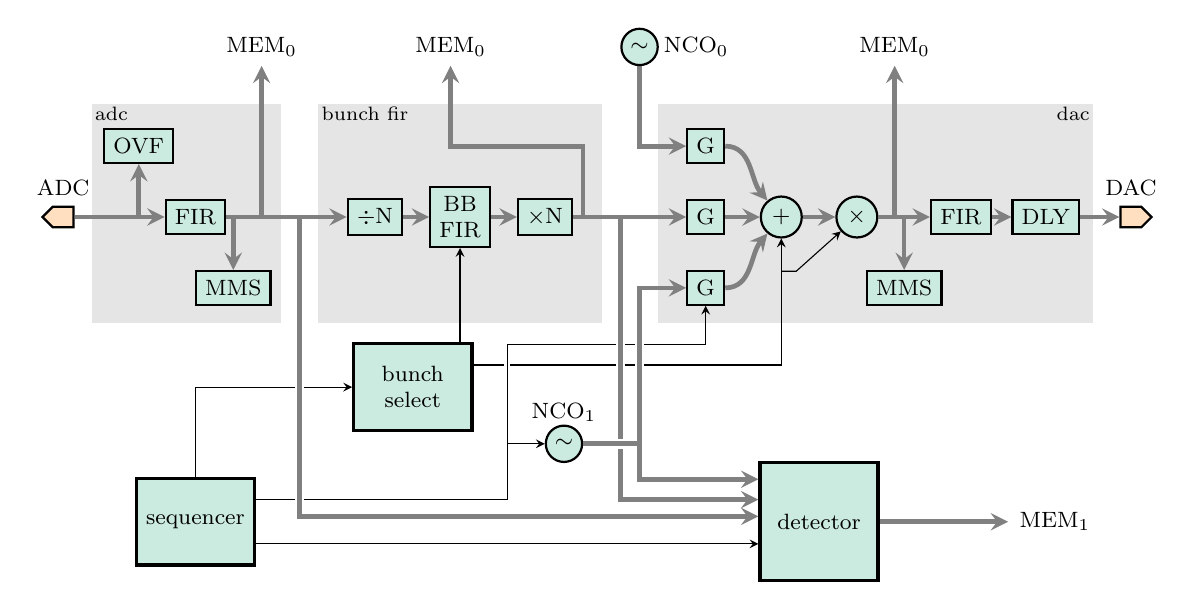
\begin{tikzpicture}[
    adc-dac/.style={
        draw, single arrow, thick, accent fill,
        single arrow head extend=0pt, shape border rotate=#1},
    area label/.style={anchor=north west, font=\scriptsize, inner sep=1pt},
    mul/.style={
        draw=black, circle, thick, highlight fill, inner sep=0.5ex},
    every node/.append style={font=\footnotesize},
    control mux/.style={
        small box, accent fill, label={[font=\tiny]above:MUX}, font=\tiny},
    x=12mm, y=9mm
    ]

    \path [background fill] (0.3,1.6)
        node [area label] {adc} rectangle ++(2,-3.1);
    \path [background fill] (2.7,1.6)
        node [area label] {bunch fir} rectangle ++(3.0,-3.1);
    \path [background fill] (6.3,1.6) rectangle ++(4.6,-3.1)
        ++(0,3.1) node [area label, anchor=north east] {dac};

    \path
        (0,0) node [adc-dac=180, label={ADC}] (adc in) {}
        +(0.8,1) node [small box] (adc ovf) {OVF}
        ++(1.4,0) node [small box] (adc fir) {FIR}
        +(0.4,-1) node [small box] (adc mms) {MMS}
        +(0.7,2.4) node (adc mem) {MEM\textsubscript{0}}
        ++(1.9,0) node [small box] (decimate) {$\div$N}
        ++(0.9,0) node [small box] (bb fir) {BB\\FIR}
        ++(0.9,0) node [small box] (interpolate) {$\times$N}
        +(-1,2.4) node (fir mem) {MEM\textsubscript{0}}
        ++(1.7,0) node [small box] (fir gain) {G}
        +(0,1) node [small box] (nco0 gain) {G}
        +(0,-1) node [small box] (nco1 gain) {G}
        ++(0.8,0) node [mul] (sum) {$+$}
        ++(0.8,0) node [mul] (product) {$\times$}
        +(0.5,-1) node [small box] (dac mms) {MMS}
        +(0.4,2.4) node (dac mem) {MEM\textsubscript{0}}
        ++(1.1,0) node [small box] (dac fir) {FIR}
        ++(0.9,0) node [small box] (delay) {DLY}
        ++(0.9,0) node [adc-dac, label={DAC}] (dac out) {};

    \node [box] at (1.4,-4.3) (sequencer) {sequencer};
    \path (bb fir) ++(-0.5,-2.4) node [box] (bunch) {bunch\\select};
    \node [box, minimum height=15mm] at (8,-4.3) (detector) {detector};
    \path (nco1 gain) ++(-1.5,-2.2)
        node [mul,
            label={[inner sep=1pt]above:NCO\textsubscript{1}}] (nco1) {$\sim$};

    \draw [bus] (adc in) -- (adc fir);
    \draw [bus] (adc in) -| (adc ovf);
    \draw [bus] (adc fir) -| (adc mms);
    \draw [bus] (adc fir) -| (adc mem);
    \draw [bus] (adc fir) -- (decimate);

    \draw [bus] (decimate) -- (bb fir);
    \draw [bus] (bb fir) -- (interpolate);
    \draw [bus] (interpolate) -- (fir gain);
    \draw [bus] (interpolate) ++(0.4,0) -- ++(0,1) -| (fir mem);
    \draw [bus] (fir gain) -- (sum);
    \draw [bus] (nco0 gain) to [out=0, in=130] (sum);
    \draw [bus] (nco1 gain) to [out=0, in=-130] (sum);
    \draw [bus] (sum) -- (product);
    \draw [bus] (product) -- (dac fir);
    \draw [bus] (product) -| (dac mms);
    \draw [bus] (product) -| (dac mem);
    \draw [bus] (dac fir) -- (delay);
    \draw [bus] (delay) -- (dac out);

    \draw [bus, <-] (nco0 gain) -- ++(-0.7,0) -- ++(0,1.4)
        node [mul, label={[inner sep=1pt]right:NCO\textsubscript{0}}] {$\sim$};

    \draw [thin, ->] (sequencer) |- (bunch);
    \draw [thin, ->] (bunch.north-|bb fir) -- (bb fir);
    \draw [thin, <-] (product) -- ++(-130:1) -- (\lastcoord-|sum);
    \draw [thin, ->] (bunch.20) -| (sum);
    \draw [thin, ->] (sequencer.-20) -- (\lastcoord-|detector.west);
    \draw [thin, ->] (sequencer.20) -| ($(nco1)+(-0.6,0)$)
        coordinate (nco1 control) -- (nco1);
    \multipath [thin] {\draw (nco1 control) -- ++(0,1.4);}
    \draw [thin, ->] (nco1 control) -- ++(0,1.4) -| (nco1 gain);

    \multipath [bus] {\draw (interpolate) ++(0.8,0) |- (detector.160);}
    \multipath [bus] {\draw (adc fir) ++(1.1,0) |- (detector.175);}
    \multipath [bus, -] {
        \draw (nco1) -- ++(0.8,0) -- (\lastcoord|-nco1 gain);
        \draw (nco1) -- ++(0.8,0) -- (\lastcoord|-detector.145);
    }
    \draw [bus] (nco1) ++(0.8,0) |- (nco1 gain);
    \draw [bus] (nco1) ++(0.8,0) |- (detector.145);

    \draw [bus] (detector) -- ++(2,0)
        node [anchor=west] {MEM\textsubscript{1}};

\end{tikzpicture}

% vim: filetype=tex:

\end{centering}
\caption{Overview of LMBF signal processing chain.  Key: \smallbox{OVF} ADC
input overflow detection; \smallbox{FIR} I/O compensation filter; \smallbox{MMS}
bunch position and motion measurement; \smallbox{$\div$N} decimation;
\smallbox{BB FIR} bunch by bunch filter; \smallbox{$\times$N} interpolation;
\smallbox{G} gain control; \smallbox{DLY}~output alignment delay; \smallbox[mul,
inner sep=2pt]{$\sim$} controllable oscillator.}
\end{figure*}



As noted above, the development of our new LMBF processor was driven by two
motivations: to ensure that we are ready for any new longitudinal instabilities,
and to increase the capabilities of our existing system~\cite{ipac2017rf,
ibic2016}.  We also wanted to improve our knowledge and understanding of high
speed processing hardware relevant to synchrotron diagnostics.

We started with an investigation to determine the appropriate hardware platform
for this kind of development.  Early on it was decided that we would need a
powerful FPGA with FMC (FPGA Mezzanine Card) support.  Initially we looked at
self contained FPGA platforms, and even briefly considered creating our own, but
in the end we converged on MicroTCA~\cite{mtca}.  This platform provides us with
a wide choice of crates and AMC (ATCA Mezzanine Card) processing modules with
high speed interconnect, and turns out to be compatible with a concurrent
development at DLS to develop Low Level RF with ALBA~\cite{ipac2017llrf}.

Having selected MicroTCA as our platform we then selected the following
hardware:

\begin{description}
\item[FMC-500M]
    (HPC) High Pin Count FMC providing dual channel 500\,MS/s 14-bit ADC and
    dual channel 1230\,MS/s 16-bit DAC~\cite{fmc500}.  This will support
    bunch-by-bunch operation at our machine RF frequency of 500\,MHz, and can be
    driven by our machine clock.
\item[FmcDIO5chTTLa]
    Five port digital IO FMC~\cite{fmcdio}.  This is used for miscellaneous
    triggering and other signals.
\item[AMC525]
    Double width AMC card with two HPC FMC slots, 2\,GB of fast on board DRAM,
    connected to a Virtex-7 690 FPGA, supporting an 8 lane gen3 PCIe connection
    over the MicroTCA backplane~\cite{amc525}.  This is our workhorse where all
    the FPGA firmware will run, and the fast backplane connection will allow us
    to do a lot of data processing in the associated CPU.
\item[AMC720]
    This is an AMC card with an Intex Xeon processor with ample memory and
    sufficient local storage.  We install Red Hat Enterprise Linux 7 on this,
    and run our control system and any associated signal processing.
\item[VT814]
    This is a 2U MicroTCA chassis with 6 AMC slots and dual redundant power
    supplies.
\end{description}

Fig \ref{fmc500} shows the digital processing hardware assembled ready for
insertion in the MicroTCA crate.


\section{System Design}

Fig \ref{overview} shows the signal processing chain as implemented in the
current design.  This is not so very different from figure 3 of our
ICALEPCS~2015 paper~\cite{icalepcs2015}.  The main enhancements are the improved
bunch by bunch motion measurement, longer FIR filters throughout, and rate
change to support longitudinal processing.

\subsection{Longitudinal vs Transverse Processing}





\begin{thebibliography}{99}

\bibitem{icalepcs2015}
M.G.~Abbott, G.~Rehm, I.S.~Uzun,
\emph{Architecture of Transverse Multi-Bunch Feedback Processor at Diamond},
ICALEPCS 2015

\bibitem{dipac2007}
A.F.D.~Morgan, G.~Rehm, I.~Uzun, \emph{First Tests of the Transverse Multibunch
Feedback at Diamond}, DIPAC~2007.

\bibitem{epac2008}
A.F.D.~Morgan, G.~Rehm, I.~Uzun, \emph{Performance and Features of the Diamond
TMBF System}, EPAC~2008.

\bibitem{biw2010}
G.~Rehm, M.G.~Abbott, A.F.D.~Morgan, J.~Rowland, I.~Uzun, \emph{Measurement of
Lattice Parameters Without Visible Disturbance to User Beam at Diamond Light
Source}, BIW~2010.

\bibitem{icalepcs2011}
I.~Uzun, M.G.~Abbott, M.T.~Heron, A.F.D.~Morgan, G.~Rehm, \emph{Operational
Status of the Transverse Multibunch Feedback System at Diamond}, ICALEPCS~2011.

\bibitem{ibic2013}
M.G.~Abbott, G.~Rehm, I.S.~Uzun, \emph{Capability Upgrade of the Diamond
Transverse Multibunch Feedback}, IBIC~2013.

\bibitem{ibic2014}
G.~Rehm, M.G.~Abbott, A.F.D~Morgan, \emph{New Features and Measurements using
the Upgraded Transverse Multibunch Feedback at Diamond}, IBIC~2014.

\bibitem{epac2006}
E.~Plouviez, P.~Arnoux, F.~Epaud, J.~Jacob, J.M.~Koch, N.~Michel, G.A.~Naylor,
J.\mbox{-}L.~Revol, V.~Serriere, D.~Vial, \emph{Broadband Bunch by Bunch
Feedback for the ESRF using a Single High Resolution and Fast Sampling FPGA
DSP}, EPAC~2006.

\bibitem{libera}
Instrumentation Technologies, \emph{Libera Bunch-by-Bunch},
\url{http://www.i-tech.si}.

\bibitem{ipac2017rf}
C.~Christou et al., \emph{Progress with the Diamond Light Source RF Upgrade},
IPAC~2017

\bibitem{ibic2016}
G.~Rehm, M.G.~Abbott, A.F.D.~Morgan, \emph{Measurements of Longitudinal Coupled
Bunch Instabilities and Status of New Feedback System}, IBIC~2016.

\bibitem{mtca}
MicroTCA Overview, PICMG, \url{https://www.picmg.org/openstandards/microtca/}

\bibitem{fmc500}
Innovative Integration, \emph{FMC-500, FMC Module with 2x 500 MSPS 14-bit A/D,
2x 1230 MSPS 16-bit DACs with PLL and Timing Controls},
\url{https://www.innovative-dsp.com/products.php?product=FMC-500}

\bibitem{fmcdio}
CERN Open Hardware Repository, \emph{FMC DIO 5ch TTL a},
\url{https://www.ohwr.org/projects/fmc-dio-5chttla}

\bibitem{amc525}
Vadatech, \emph{AMC525, dual FMC carrier, 2 FMC, 690T FPGA, FFG-1761 package,
FPGA Mezzanine Card}, \url{http://vadatech.com/product.php?product=393}.

\bibitem{ipac2017llrf}
P.~Gu et al., \emph{Digital Low Level RF Systems for Diamond Light Source},
IPAC~2017


\end{thebibliography}


\end{document}
